\chapter{End of chapter exercise solutions}
\label{eoceSolutions}

\begin{multicols}{2}

%%%%%%%%%%%%%%%%%%%%%%

% Chp 1
\eoceSolCh{Introduction to data}

%%%%%%%%%%%%%%%%%%%%%%

% 1
\eoceSol{(a) Control: 56\%. Treatment: 70\%. (b) There is a 14\% difference between the pain reduction rates in the two groups. It appears that patients in the treatment group are more likely to show improvement and, at a first glance, acupuncture appears to be an effective treatment for migraines. (c) It's hard to say. The difference is somewhat large, but the sample is somewhat small.}

% 3
\eoceSol{(a) 143,196 eligible subjects who were born in Southern California between 1989 and 1993. (b) The variables are measurements of CO, NO$_2$, ozone, and particulate matter less than 10$\mu$m (PM$_{10}$) collected at air-quality-monitoring stations as well as the birth weights of the babies. All of these variables are continuous numerical variables. (c) Does air pollution exposure have an effect on preterm births?'}

% 5
\eoceSol{(a) 202 black and 504 white adults who resided in or near New York City, were ages 20-94 years, and had BMIs of 18-35 kg/m$^2$. (b) Age (numerical, continuous), sex (categorical), ethnicity (categorical), weight, height, waist and hip circumference, length of tibia, body density and volume, total body water (numerical, continuous). (c) How useful is BMI for predicting body fatness across age, sex and ethnic groups?}

% 7
\eoceSol{(a) A participant in the survey. (b) 1,691 participants. (c) gender (gender of the participant), age (age of the participant, in years), marital (marital status of the participant), grossIncome (gross income of the participant, in $\pounds$), smoke (whether or not the participant smokes), amtWeekends (number of cigarettes smoked on weekend, \# of cigarettes / day), amtWeekdays (number of cigarettes smoked on a week day, \# of cigarettes / day).}

% 9
\eoceSol{gender (categorical), age (originally numerical, continuous, though it was recorded as a discrete numerical variable), maritalStatus (categorical), grossIncome (originally numerical, continuous, but recorded as categorical), smoke (categorical), amtWeekends (numerical, discrete), amtWeekdays (numerical, discrete).}

% 11
\eoceSol{We would expect productivity to increase as stress increases, but up to a point, after that productivity would decrease as stress continued to increase. The exact shape of your plot may be a little different. \vspace{-3mm}\\
\includegraphics[width = 0.29\textwidth]{01/figures/eoce/StressProductivity.pdf}\vspace{-3mm}
}

% 13
\eoceSol{(a) Population mean, $\mu_x = 5.5$; sample mean, $\bar{x} = 6.25$. (b) Population mean, $\mu_x = 52$; sample mean, $\bar{x} = 58$.}

% 15
\eoceSol{(a) Decrease. (b) 73.6. (c) The new score, $x_{25}$, is more than 1 standard deviation away from the previous mean, and this will tend to increase the standard deviation of the data. While possible, it is mathematically rather tedious to calculate the new standard deviation.}

% 17
\eoceSol{The distribution of amount of cigarettes smoked on weekends and on weekdays are both right skewed. The median of both distributions is between 10 and 15 cigarettes, the first quartile is between 5 and 10 cigarettes, and the third quartile is between 15 and 20 cigarettes. Hence the IQR of both distributions is roughly about 10 cigarettes. There are potential outliers above 40 cigarettes per day, giving both distributions a long right tail. We can also see that there are more respondents who smoke only a few cigarettes (0 to 5) on the weekdays, about 80 people, than on weekends, about 60 people. Another feature that is visible from the histograms are peaks at 10 and 20 cigarettes. This may be because most people do not keep track of exactly how many cigarettes they smoke, but round their answers to half a pack (10 cigarettes) or a whole pack (20 cigarettes). Due to these peaks, the distributions could be classified as bimodal.}

% 19
\eoceSol{$s_{amtWeekends} = 0, s_{amtWeekdays} = 4.18$. Variability of the amount of cigarettes smoked is higher on weekdays than on the weekends for this sample.}

% 21
\eoceSol{(a) 6 (b) 6.5}

% 23
\eoceSol{Plot below. \\
\includegraphics[width = 0.44\textwidth]{01/figures/eoce/StatsFinalScoresBoxplot.pdf}\vspace{-2mm}
}

% 25
\eoceSol{(a) The distribution is unimodal and symmetric with a mean around 60 and a standard deviation of roughly 3; matches the box plot (2). (b)The distribution is uniform and values range from 0 to 100; matches box plot (3) which shows a symmetric distribution in this range. Also, each 25\% chunk of the box plot have about the same width and there are no suspected outliers. (c) The distribution is unimodal and right skewed with a median between 1 and 2. The IQR of the distribution is roughly 1; matches box plot (1).}

% 27
\eoceSol{(a) Since median is defined as the $50^{th}$ percentile and about 50\% of the data is in the first bar, we would expect median to be between 0 and 20. Q1 is also between 0 and 20 as the $25^{th}$ percentile is in the first bar as well. Q3, defined as the $75^{th}$ percentile, is located between 40 and 60. (b) The distribution is right-skewed, so the long tail will pull the mean above the median.}

% 29
\eoceSol{It appears that marathon times decreased greatly between 1970-1975 and remained somewhat steady thereafter. Males consistently had shorter marathon times than females throughout the years. From the box plots of males and females, we could tell that males ran faster ``on average", however, we could not tell that the winning male time for each year was better than the winning female time. We also could not tell from the histogram or the box plot that marathon times have been decreasing for males and females throughout the years.}

% 31
\eoceSol{(a) The distribution is right skewed with potential outliers on the positive end, therefore the median and the IQR are appropriate measures of center and spread. (b) The distribution is somewhat symmetric and probably does not have outliers, therefore the mean and the standard deviation are appropriate measures of center and spread. (c) The distribution would be right skewed. There would be some students who do not consume any alcohol but this is the minimum (there cannot be students who consume fewer than 0 drinks). There would be a few students who consume many more drinks than their peers, giving the distribution a long right tail. Due to the skew, the median and the IQR would be appropriate measures of center and spread. (d) The distribution would be right skewed. Most employees would make something on the order of the median salary, but we would expect to have some high level executives making a lot more. The distribution would have a long right tail, and the median and the IQR would be more more appropriate measures of center or spread.}

% 33
\eoceSol{(a) As well as the order of the categories, we can also see the relative frequencies in the bar plot. These proportions are not readily available in the pie chart. (b) None. (c) Bar plot, so that we can also see the relative frequencies of the categories in this graph.}

% 35
\eoceSol{(a) Proportion of patients who are alive at the end of the study is higher in the treatment group than in the control group. Therefore survival is not independent of whether or not the patient got a transplant. (b) The shape of the distribution of survival times in both groups is right skewed with outliers on the high end. The median survival time for the control group is much lower than the median survival time for the treatment group; patients who got a transplant typically lived longer. The maximum survival time for the treatment group is much higher (about 5 years) than the maximum survival time for the control group. Even though the maximum survival time for the control group is about 4 years, this observation is an outlier. Overall, very few patients without transplants made it beyond a year while nearly half of the transplant patients survived at least one year. It should also be noted that while the first and third quartiles of the treatment group is higher than those for the control group, the IQR for the treatment group is much bigger, indicating that there is more variability in survival times in the treatment group.}

% 37
\eoceSol{(a) The population is all adults 20 and older living in the greater New York City area. The sample is the 202 black and 504 white men and women who resided in or near New York City and had BMIs of 18-35 kg/m$^2$. (b) The population is all Californians registered to vote in the 2010 midterm elections. The sample is the 1000 registered California voters who were surveyed for this study.}

% 39
\eoceSol{(a) This is an observational study. (b) Wealth is one lurking variable. Countries with individuals who can widely afford internet probably also can afford basic medical care. (Note: Answers may vary.)}

% 41
\eoceSol{(a) Simple random sample. Non-response bias, if only those people who have strong opinions about the survey responds his sample may not be representative of the population. (b) Convenience sample. Under coverage bias, his sample may not be representative of the population since it consists only of his friends.}

% 43
\eoceSol{(a) Non-responders are most likely parents who have busier schedules and have difficulty spending time with their kids after school. (b) The women who are not reached 3 years later are most likely renters (as opposed to homeowners) who may be in a lower socio-economic status. (c) There is no control group and there may be lurking variables. For example, it may be that these people who go running are generally healthier and/or do other exercises.}

% 45
\eoceSol{No, this was an observational study, and we cannot make such a causal statement based on an observational study.}

% 47
\eoceSol{Prepare two cups for each participant one containing regular Coke and the other containing Diet Coke. Make sure the cups are identical and contain equal amounts of soda. Label the cups A (regular) and B (diet). (Be sure to randomize A and B for each trial!) Give each participant the two cups, one cup at a time, in random order, and ask the participant to record a value that indicates how much she liked the beverage.  Be sure that neither the participant nor the person handing out the cups knows the identity of the beverage to make this a double-blind experiment. (Answers may vary.).}

% 49
\eoceSol{(a) Experiment. (b) Treatment: exercise twice a week, control: no exercise. (c) Yes, the blocking variable is age. (d) No. (e) Since this is an experiment, we can make a causal statement. Since the sample is random, the causal statement can be generalized to the population at large. However, we should be cautious about making a causal statement because of a possible placebo effect. Note that this study could not actually be conducted since people cannot be required to participate in a clinical trial.
}

% 51
\eoceSol{(a) False. Instead of comparing counts, we should compare percentages of people in each group who suffered a heart attack. (b) True. (c) False. Association does not imply causation. We cannot infer a causal relationship based on an observational study. (We cannot say changing the drug a person is on affects her risk, which is why part (b) is true.) (d) True.}

\noindent\rule{0.48\textwidth}{0.5mm}\vspace{-3mm}
\noindent\rule{0.48\textwidth}{0.5mm}

\addvspace{3mm}

%%%%%%%%%%%%%%%%%%%%%%

% Chp 2
\eoceSolCh{Probability}

%%%%%%%%%%%%%%%%%%%%%%

%1
\eoceSol{False. The tosses are independent trials.}

%3
\eoceSol{(a) 10 tosses. With a low number of flips the variability in the number of heads observed is much larger, so a result further from 50\% is more likely. (b) 100 tosses. With more flips, the observed proportion of heads would probably be closer to 50\% and therefore above 40\%. (c) 100 tosses. The more flips, the less variability away from 50\%. (d) 10 tosses. Fewer flips mean more volatility and a greater chance of getting far from 50\% and below 30\%.}

%5
\eoceSol{(a) $1/1024$. (b) $1/1024$. (c) $1023/1024$.}

%7
\eoceSol{(a) Figure below. (b) 5\% (c) 70\% (d) 95\% (e) 5\% (f) No, there are bloggers who own both types of cameras. \\
\includegraphics[width=0.4\textwidth]{02/figures/eoce/psDslrVenn.png}
}

%9
\eoceSol{(a) Not mutually exclusive. If the class is not graded on a curve, then independent. If graded on a curve, dependent. (b) Not mutually exclusive, most likely dependent. (c) No. See the answer to (a) when the course is not graded on a curve.}

%11
\eoceSol{(a) 0.26. (b) 0.23. (c) Assuming that the education level of the husband and wife are independent, 0.0598. (d) Independence, which may not be a reasonable assumption since people often marry others with a comparable level of education.}

%13
\eoceSol{(a) Sum greater than 1. (b) OK mathematically. (c) Sum less than 1. (d) Negative probabilities make no sense. (e) OK. (f) Probabilities cannot be less than 0 or greater than 1.}

%15
\eoceSol{Approximate answers are OK. Answers are only estimates based on the sample. (a) 0.42. (b) 0.15. (c) 0.37. (d) 0.06.}

%17
\eoceSol{(a) The distribution is right skewed, with a median between \$35,000 and \$49,999. The IQR of the distribution is about \$27,500. There are probably outliers on the high end due to the nature of the data. (b) 62.2\%. (c) Assuming gender and income are independent: 25.5\%. (d) P(less than \$50,000 and female) = 29.4\%. The independence assumption does not appear to be valid. If gender and income were independent, we would expect the 25.5\% of the sample to be female and make less than \$50,000, but actually a higher proportion fall into this category.}

%19
\eoceSol{No, P(DSLR $|$ point\&shoot) = 0.22, which is not equal to P(DSLR).}

% 21
\eoceSol{(a) 0.2825. (b) 0.1905. (c) 0.4167. (d) No, because P(black hair $|$ brown eyes) $\ne$ P(black hair $|$ blue eyes). (Other explanations are possible.)}

% 23
\eoceSol{(a) 0.65. (b) 0.72. (c) Under the assumption of independence of gender and hamburger preference: 0.468. While it is possible there is some mysterious connection between burger choice and finding a partner, independence is probably a reasonable assumption. (e) 0.514.}

% 25
\eoceSol{Female, most cats smaller than 2.5kg are female.}

% 27
\eoceSol{0.6049.}

% 29
\eoceSol{(a) Tree diagram below. (b) 0.68. (c) 0.32. (d) Your test results have come in. While the test came back positive, this is not conclusive. A positive test result can occur even when a patient has no disease; occasionally a test will be wrong. For this reason, we will need to run some additional tests. \\
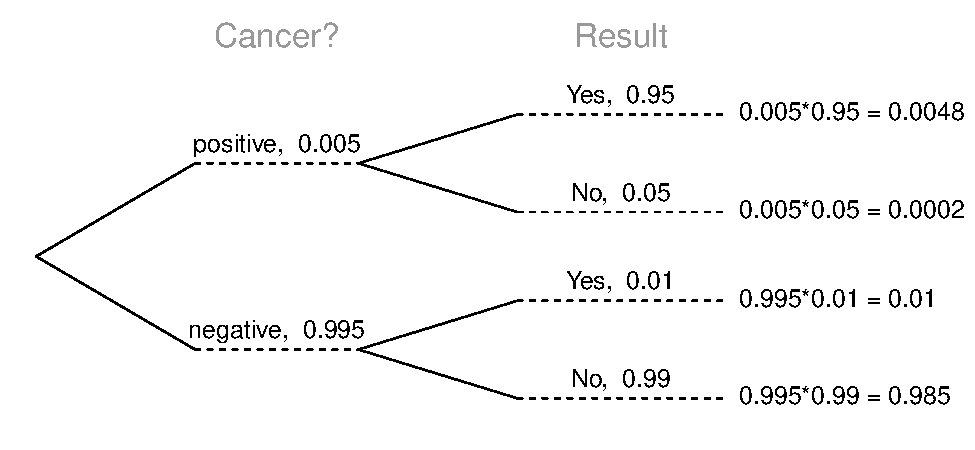
\includegraphics[width=0.45\textwidth]{02/figures/eoce/cancerTree.pdf}}

% 31
\eoceSol{(a) 0.3. (b) 0.3. (c) 0.3. (d) 0.09. (e) Yes, each draw is from the same set of marbles.}

% 33
\eoceSol{(a) 0.0909. (b) 0.3182. (c) 0.4545. (d) 0. (e) 0.2879.}

% 35
\eoceSol{0.0519.}

% 37
\eoceSol{(a) 13. (b) No, this would be unreliable. The students are not a random sample.}

% 39
\eoceSol{(a) Table below. Expected winnings: \$3.59. SD: 3.37. (b) EV: -\$1.41, SD: \$3.37. (c) No. The expected net profit is negative, so on average you expect to lose money. \\
{\scriptsize\begin{tabular}{llll}
&&&\\
\hline
Event	& 3 hearts & 3 blacks & Else \\
\hline
$X$		& \$50	& \$25	& \$0 \\
$P(X)$	& 0.0129	& 0.1176	& 0.8695 \\
$X * P(X)$	& 0.65 & 2.94	& 0 \\
$(X \hspace{-0.5mm} - \hspace{-0.5mm} E(X))^2  P(X)$ & 0.1115	& 0.0497	& 11.2062\hspace{-0.75mm} \\
\hline
&&&\\
\end{tabular}}}

% 41
\eoceSol{(a) EV: -\$0.16, SD: \$2.99. (b) EV: -\$0.16, SD: \$1.73. (c) Expected values are the same but the standard deviations are different. The standard deviation from the game where winnings and losses are tripled is higher, making this game riskier.}

% 43
\eoceSol{(a) Table to the right. Expected winnings: -\$0.54 (b) No, he is expected to lose money on average. \\
{\scriptsize\begin{tabular}{lllll}
\hline
Event	& 2,...,9	& J, Q, K	& Ace	& A$\clubsuit$ \\
\hline
$X$		& -2		& 1		& 3		& 23 \\
$P(X)$	& 0.6923	& 0.2308	& 0.0577	& 0.0192 \\
\hline
\end{tabular}}}

% 45
\eoceSol{\$4.26.}

% 47
\eoceSol{(a) Mean: \$3.90, SD: \$0.34. (b) Mean: \$27.30, SD: \$0.89.}

\noindent\rule{0.48\textwidth}{0.5mm}\vspace{-3mm}
\noindent\rule{0.48\textwidth}{0.5mm}

\addvspace{3mm}

%%%%%%%%%%%%%%%%%%%%%%

% Chp 3
\eoceSolCh{Distributions of random variables}

%%%%%%%%%%%%%%%%%%%%%%

% 1
\eoceSol{Plots below. (a) 0.0885. (b) 0.0694. (c) 0.5886. (d) 0.0456.}
\noindent
\includegraphics[width=0.245\textwidth]{03/figures/eoce/zltNeg}
\includegraphics[width=0.245\textwidth]{03/figures/eoce/zgtPos}
\includegraphics[width=0.245\textwidth]{03/figures/eoce/zBet}
\includegraphics[width=0.245\textwidth]{03/figures/eoce/zgtAbs}

% 3
\eoceSol{(a) Verbal: $N(\mu = 462, \sigma = 119)$, Quant: $N(\mu = 584, \sigma = 151)$. (b) $Z_{VR} = 1.33$, $Z_{QR} = 0.57$. Plots below. (c) She scored 1.33 standard deviations above the mean on the Verbal Reasoning section and 0.57 standard deviations above the mean on the Quantitative Reasoning section. (d) Perc$_{VR}=91\%$, Perc$_{QR}=72\%$. (e) Verbal Reasoning. (f) VR: 9\%, QR: 28\%. (g) We cannot compare the raw scores since they are on different scales. Her scores will be measured relative to the merits of other students on each exam, so it is helpful to consider the Z score. Comparing her percentiles is more appropriate for determining how well she did compared to others. \\
\includegraphics[width=0.4\textwidth]{03/figures/eoce/GRE}}

% 5
\eoceSol{Answers to (b) and (c) would not change, though we would not draw a Normal curve on which to show these scores. We could not answer parts (d) and (e) since the normal probability table is only valid for the normal model.}

% 7
\eoceSol{(a) 711. (b) 400.}

% 9
\eoceSol{Figures below. (a) 0.1210. (b) 0.1558. (c) 62.68 inches. (d) 43.25\%}
\noindent
\includegraphics[width=0.24\textwidth]{03/figures/eoce/heightLt48}
\includegraphics[width=0.24\textwidth]{03/figures/eoce/heightBet}
\includegraphics[width=0.24\textwidth]{03/figures/eoce/heightPerc}
\includegraphics[width=0.24\textwidth]{03/figures/eoce/heightLt54}

% 11
\eoceSol{(a) 0.1401. (b) 70.6$^o$F or colder.}

% 13
\eoceSol{(a) 0.67. Using 0.68 is also okay, but your answers for part (c) will differ a little from the listed solution. (b) $x=\$1800$, $\mu=\$1650$. (c) $\sigma=\$223.88$.}

% 15
\eoceSol{(a) 0.2327. Figure below. (b) If you are bidding on only one auction and set a maximum bid price that is too low, chances are someone will outbid you and you won't win the auction. If your maximum bid price is too high, you may win the auction but you may be paying more than is necessary. If you are bidding on more than one auction and your maximum bid price is too low, chances are you won't win any of the auctions. However, if your maximum bid price is too high, you may win more than one auction and end up with multiple copies of the book. (c) An answer roughly equal to the 10$^{th}$ percentile would be reasonable. Regrettably, no percentile cutoff point guarantees beyond any possible event that you win at least one auction. However, you may pick a higher percentile if you want to be more sure of winning an auction. (d) Using the 10$^{th}$ percentile: \$69.80. Answers may vary but should correspond to the answer given in part (c). \\
\includegraphics[width=0.4\textwidth]{03/figures/eoce/chemBooks1}}

% 17
\eoceSol{70\% of the data are within 1 SD, 95\% are within 2 SD, and 100\% are within 3 SD of the mean. The data approximately follow the 68-95-99.7\% Rule.}

% 19
\eoceSol{The distribution is unimodal, symmetric, and approximately follows the 68-95-99.7\% Rule. The superimposed normal curve seems to approximate the distribution pretty well. The points on the Normal probability plot also seem to follow a straight line. There is one possible outlier on the lower end that is apparent in both graphs, but it is not too extreme. We can say that the distribution is nearly normal.}

% 21
\eoceSol{No, in poker cards are dealt without replacement, and they have more than two categories.}

% 23
\eoceSol{Approximate answers are OK. (a) 0.13. (b) 0.12. (c) $\mu= 2.04 $, $\sigma= 1.46 $. (d) $\mu= 3.33 $, $\sigma= 2.79$. (e) When $p$ was smaller, i.e. the event was rarer, the expected number of trials before a success and the standard deviation increased.}

% 25
\eoceSol{(a) 0.096. (b) $\mu=8$, $\sigma= 7.48$.}

% 27
\eoceSol{(a) Yes, it meets the four required conditions. (b) 0.203. (c) 0.203. (d) 0.167. (e) 0.997.}

% 29
\eoceSol{(a) $\mu=34.85$, $\sigma=3.25$. (b) Yes, since 45 is more than 3 standard deviations from the mean. (c) 0.0015 (an answer of 0.0009 would be okay if using a normal approximation, since the conditions for the approximation are satisfied). In part (b), we had determined that it would be unusual to observe 45 or more 18-20 year olds who have consumed alcoholic beverages among a random sample of 50, and the we calculated a very low probability for this event.}

% 31
\eoceSol{(a) 0.5160. (b) 0.1234. (c) 0.8483. (d) No, otherwise there is a 15.17\% chance that 2 or more will be afraid of spiders in any particular tent.}

% 33
\eoceSol{(a) 0.109. (b) 0.219. (c) 0.137. (d) 0.551. (e) 0.084. (f) Since 2 is $\frac{2 - 4}{1.06} = -1.89$ standard deviations below the expected number of brown eyed children, strictly speaking this would not be considered unusual. However, it should be noted that the z-score for this value is pretty close to 2, making this observation borderline unusual.}

% 35
\eoceSol{The probability model is below. \vspace{-1.5mm}
\begin{center}\scriptsize
\begin{tabular}{lllll}
\hline
$Y$	& -3	& -1	& 1	& 3 \\
$P(Y)$	& 0.1458	& 0.3936	& 0.3543	& 0.1063 \\
\hline
\end{tabular}
\end{center}}

% 37
\eoceSol{(a) (1/5)*(1/4)*(1/3)*(1/2)*(1/1) = 1/(5!) = 1/120. (e) 120 = 5!. (c) 8! = 40,320.}

% 39
\eoceSol{(a) 0.0804 using the geometric distribution. (b) 0.0322 using the binomial distribution. (c) 0.0193 using the negative binomial distribution.}

% 41
\eoceSol{(a) Negative Binomial (n = 4, p = 0.55): Of the four trials considered here, the last trial must be a success and there were exactly 2 successes. (b) 0.1838. (c) ${3\choose1} = \frac{3!}{2!1!} = 3$. (d)  In the binomial model we have no restrictions on the outcome of the last trial while in the negative binomial model the last trial is fixed. Therefore we are interested in the number of ways of orderings of the other $k - 1$ successes in the first $n - 1$ trials.}

% 43
\eoceSol{(a) Poisson with $\lambda=75$. (b) $\mu=\lambda=75$, $\sigma=\sqrt{\lambda} = 8.66$. (c) No, since 60 is within 2 standard deviations of the mean.}

% 45
\eoceSol{$P(X = 70) = \frac{75^{70} e^{-75}}{70!} = 0.0402$}


\noindent\rule{0.48\textwidth}{0.5mm}\vspace{-3mm}
\noindent\rule{0.48\textwidth}{0.5mm}

\addvspace{3mm}

%%%%%%%%%%%%%%%%%%%%%%

% Chp 4
\eoceSolCh{Foundations for inference}

%%%%%%%%%%%%%%%%%%%%%%

% 1
\eoceSol{(a) Mean. (b) Mean. (c) Proportion. (d) Mean. (e) Proportion.}

% 3
\eoceSol{The point estimates are the corresponding sample values. (a) $\bar{x}=13.65$, median$=14$. (b) $s=1.91$, $IQR_{estimate} = 2$. (c) Use the Z score to evaluate ($Z_{16} = 1.23$, $Z_{18} = 2.28$), so 18 credits is unusually high but 16 is not, where we use 2 standard deviations from the mean as a cutoff for deciding what is unusual.}

% 5
\eoceSol{No, sample point estimates only approximate the population parameter, and they vary from one sample to another.}

% 7
\eoceSol{Standard error, $SE_{\bar{x}} = \frac{1.91}{\sqrt{100}} = 0.191$.}

% 9
\eoceSol{(a) $SE_{\bar{x}} = 2.89$ (b) The Z score is 1.73 (absolute value is less than 2), so \$80 is consistent.}

% 11
\eoceSol{(a) Independence is met by the random sampling assumption and that the sample is less than 10\% of the population. The sample size is also sufficiently large. We cannot check the assumption that the distribution isn't extremely skewed. (b) (19.862, 20.058). (c) We are 90\% confident that the true mean amount of coffee in Starbucks venti cups is between 19.862 ounces and 20.058 ounces. (d) 90\% of random samples of size 50 will yield confidence intervals that capture the true mean amount of coffee in Starbucks venti cups. (e) Yes, 20 ounces is included in the interval. (f) A 95\% confidence interval would be wider. All else kept constant, when confidence level increases so does the margin of error and hence the interval becomes wider. We cast a wider interval.}

% 13
\eoceSol{(a) Less. (b) We can infer from the sample statistics that the distribution is skewed, so no we cannot. (c) The only condition that may not be met for normality of the mean relates to skew: it is unclear if the distribution is extremely skewed or not. We'll suppose the skew is strong but not too extreme, something we may like to look into further. Solution: 0.0985. (d) Decreases the standard error by a factor $\sqrt{2}$.}

% 15
\eoceSol{When the confidence level increases, so does the margin of error and the width of the interval. A wide interval may be undesirable even if the confidence level is higher.}

\vspace{3mm}

% 17
\eoceSol{(a) False, since we need only check whether the skew is not too extreme. (b) False, we are 100\% sure the average for \emph{these} patients is in this interval. (c) True. (d) False, the confidence interval is not about sample means. (e) False, as the confidence level increases, so does the width of the interval. (f) True. (g) False, since in calculation of the standard error we divide the standard deviation by square root of the sample size, we would need to quadruple the sample size.}

% 19
\eoceSol{(a) 0.0004. (b) Since the sample is random and the 10\% condition is met, we can assume the that how much one penny weighs is independent of another. Since the population distribution is normal, and hence not extremely skewed, sampling distribution of means will be nearly normal even though $n < 50$. $N(\mu=2.5, \sigma_{\bar{x}} = 0.0095)$. (c) Approximately 0. (d) Plot below. (e) The sample or sampling distributions would not be approximately normal.
\begin{center}
\includegraphics[width=0.485\textwidth]{04/figures/eoce/pennies3}
\end{center} 
}

% 21
\eoceSol{(a) From the histogram: $P(X > 5) = \frac{350 + 100 + 25 + 20 + 5}{3000} = \frac{500}{3000} = 0.17$. It's okay if your answer differs a little. (b) Two different answers are reasonable. 1) The conditions are reasonably met. We know the population standard deviation, so we can know the standard error (SD of $\bar{x}$) with certainty. The population distribution is also only slightly skewed, so a sample of 15 would probably have a sampling distribution for the mean that is nearly normal. Solution: 0.0956. 2) If you had said the normality condition for $\bar{x}$ was questionable because the population distribution was not normal, that is also an acceptable answer. (c) Assumptions/conditions are certainly met. Solution: 0.1788.}

\vspace{3mm}

% 23
\eoceSol{(a) $H_0$: $\mu = 8$ (On average New Yorkers sleep 8 hrs a night), $H_A$: $\mu < 8$ (On average New Yorkers sleep less than 8 hrs a night). (b) $H_0$: $\mu = 15$ (The average amount of company time spent not working is 15 minutes), $H_A$: $\mu > 15$ (The average amount of company time spent not working is greater than 15 minutes).}

% 25
\eoceSol{The hypotheses should be about the population mean ($\mu$), not the sample mean. If he believes that \$1.3 million is an overestimation, the alternative hypothesis should be \emph{less than} and not \emph{greater than}. The correct way to set up these hypotheses is as follows: $H_0$: $\mu = \$1.3~million$, $H_A$: $\mu < \$1.3~million$.}

% 27
\eoceSol{(a) 180 minutes is not in the interval, so this is implausible. (b) 2.2 hours (132 minutes) is in the interval, so we conclude the estimated wait time of 2.2 hours is reasonable. (c) A 99\% confidence interval will be wider than a 95\% confidence interval. Hence even without calculating the interval we can tell that 132 minutes would be in it.}

% 29
\eoceSol{(a) $H_0$: Anti-depressants do not work for the treatment of Fibromyalgia. $H_A$: Anti-depressants work for the treatment of Fibromyalgia. (b) Concluding that anti-depressants work for the treatment of Fibromyalgia when they actually do not. (c) Concluding that anti-depressants do not work for the treatment of Fibromyalgia when they actually do. (d) If she makes a Type I error, she will continue taking medication that does not actually treat her disorder. If she makes a Type II error, she will stop taking medication that could treat her disorder.}

% 31
\eoceSol{(a) Yes, if we assume there isn't too much skew, which is certainly reasonable once we realize the possible percentages, which must be between 0\% and 100\%, are bounded within 3 standard deviations from the mean. (b) $H_0$: $\mu = 0.25$, $H_A$: $\mu \ne 0.25$. $Z = -7.71 \to $ two-sided p-value $\approx 0$. Reject $H_0$: the evidence indicates that the percentage of time college students spend on the internet for coursework has changed over the last decade. (c) If the percentage of time college students spend on the Internet for course work has actually remained at 25\%, the probability of getting a random sample of 238 college students where the average percentage of time they spend on the Internet for course work is 10\% or less or 40\% or more is approximately 0. (d) Type I, since we may have incorrectly rejected $H_0$.}

% 33
\eoceSol{$H_0$: $\mu = 7$, $H_A$: $\mu \ne 7$. $Z=-1.04\to$single tail$=0.1492\to$ p-value $=2*0.1492=0.2984$. There isn't sufficient evidence that the average lifespan of all ball bearings produced by this machine is not 7 hours. The manufacturer's claim is not implausible.}

% 35
\eoceSol{$\bar{x} = 36.05$.}

% 37

\eoceSol{(a) The distribution is unimodal and right skewed, median is between 5 and 10 years old, and the IQR is roughly 10. There are potential outliers on the higher end. (b) When the sample size is small, the sampling distribution is right skewed, just like the population distribution. As the sample size increases, the sampling distribution gets more and more unimodal and symmetric, just like the CLT suggests.}

% 39
\eoceSol{(a) If the skew is not too strong, the assumptions are met. (b) $H_0$: $\mu = 432$, $H_A$: $\mu < 432$. $Z=-3.28 \to$ p-value (single tail) $=0.0005$. Since the p-value $< \alpha$, we reject $H_0$. There is evidence that the average amount savings of all customers who switch their insurance is less than \$432. (c) Yes, the insurance company's claim may be an overestimate since the hypothesis test result indicated there was strong evidence that the average savings is less than the advertised amount. (d) (\$376.47, \$413.53). (e) Yes, the hypothesis test was statistically significant and \$432 was not in the confidence interval.}

% 41
\eoceSol{(a) The only condition we cannot check is for extreme skew. Here, we will assume this is not an issue; in practice, this is something we should verify. (b) $H_0$: $\mu = 500$, $H_A$: $\mu \ne 500$. $Z=-3.86 \to$single tail$\approx 0\to$ p-value $\approx 2*0=0$. Since the p-value $< \alpha$ (0.05), we reject $H_0$. The data provide strong evidence that the average increase in reading speed is not 500\% (it is below 500\% based on the data). (c) No, the company's claim of an average of 500\% increase in reading speed does not appear to be accurate. (d) 371.88\% to 458.12\%. (e) Yes. The hypothesis test rejected that the average increase was 500\%, and 500\% was not in the confidence interval.}

% 43

\eoceSol{$n \ge 693$.}

\noindent\rule{0.48\textwidth}{0.5mm}\vspace{-3mm}
\noindent\rule{0.48\textwidth}{0.5mm}

\addvspace{3mm}

%%%%%%%%%%%%%%%%%%%%%%

% Chp 5
\eoceSolCh{Large sample inference}

%%%%%%%%%%%%%%%%%%%%%%

% 1
\eoceSol{(a) Hypothesis test for paired data. (b) $H_0$: $\mu_{diff} = 0$ (There is no difference in average daily high temperature between January 1, 1968 and January 1, 2008), $H_A$: $\mu_{diff} > 0$ (Average daily high temperature in January 1, 1968 was lower than average daily high temperature in January, 2008.) (c) Independence is satisfied since we have a random sample that is less than 10\% of the possible locations we could collect such measurements in the continental U.S. There is also a one-to-one correspondence between the observations in the data set, making it appropriate for a paired analysis. The sample size is sufficiently large ($n=51$). If we had the data in hand, we would also check for extreme skew. $Z = 1.60$, p-value $= 0.0548$. (d) Fail to reject $H_0$. The data do not provide strong evidence of temperature warming in the continental US. However, it should be noted that the p-value is very close to 0.05. (e) Type II. If we made such an error and concluded that there isn't strong evidence for temperature warming in the continental US, but in reality average temperature on January 1, 2008 is higher than average temperature on January 1, 1968. (f) Yes.}

% 3
\eoceSol{(a) $H_0$: $\mu_{B} = \mu_{A}$, another way to write this is $\mu_{B} - \mu_{A} = 0$ (The population mean of number of cigarettes smoked per day did not change after the Surgeon General's report), $H_A$: $\mu_1 > \mu_2$, another way to write this is $\mu_1 - \mu_2 > 0$ (The population mean of number of cigarettes smoked per day decreased after the Surgeon General's report) (b) Independence is satisfied since we have two random samples that are less than 10\% of their respective populations. The sample sizes are sufficiently large. If we had the data in hand, we would also check for extreme skew. $Z = 1.89$, p-value $= 0.0294$. (c) Reject $H_0$. There is sufficient evidence that the number of cigarettes smoked per day decreased after the Office of the Surgeon General's report. (d) No, we cannot make a causal connection because this is observational data. (e) Type I, since we may have incorrectly rejected $H_0$.}

% 5
\eoceSol{Independence is satisfied since we have two independent random samples that are each less than 10\% of the population. The sample sizes are sufficiently large. If we had the data in hand, we would also check for extreme skew. We are 90\% confident that the average score in 2004 was 0.16 to 5.84 points lower than the average score in 2008.}

% 7
\eoceSol{$H_0$: $\mu_M = \mu_W$, $H_A$: $\mu_M < \mu_W$. $Z = -97.35$, p-value $\approx 0$. Reject $H_0$. The data provide strong evidence that average body fat percentage for women is higher.}

% 9
\eoceSol{(a) False, for proportions need to check success/failure condition, not $n \ge 50$. (b) True. (c) False, only 1.65 standard errors away from the mean, and we use 2 as a cutoff for what is called unusual. (d) True. (e) False, standard error would decrease only by a factor of $\sqrt{2}$.}

% 11
\eoceSol{(a) True. (b) False, standard error would decrease only by a factor of $\sqrt{2}$. (c) True. (d) True. (e) False, success/failure condition is not satisfied.}

% 13
\eoceSol{(a) Paremeter: proportion of all graduates from this university who found a job within one year of graduating. Point estimate: 0.87. (b) Independence is satisfied since we have a random sample that is less than 10\% of the population. Normality is satisfied since the success-failure condition is met. CI: (0.837 , 0.903). (c) We are 95\% confident that the true proportion of graduates from this university who found a job within one year of completing their undergraduate degree is between 83.7\% and 90.3\%. (d) 95\% of random samples of 400 would produce a confidence interval that includes the true proportion of students at this university who found a job within one year of graduating from college. (e) It would be wider. (f) It would be narrower.}

% 15
\eoceSol{(a) She needs a minimum of 3,394 subjects and therefore needs to set aside a minimum of \$67,880. (b) It will be wider.}

% 17
\eoceSol{(a) $ME = 1.96 * \sqrt{0.66 * 0.34 / 1,1018} \approx 0.03$. (b) No, for two reasons. The point estimate is slightly below 67\%, and 67\% is contained in the interval.}

% 19
\eoceSol{(a) $H_0$: $p = 0.5$, $H_A$: $p > 0.5$. Assuming the sample is random. The sample is simple random and from $<$10\% of the population, so independence is reasonable. The success/failure condition is also met. $Z = 4.66$, p-value $\approx 0$. Since the p-value is small, we reject $H_0$. The data provide strong evidence that majority of the Americans think the Civil War is still relevant. (b) If in fact only 50\% of Americans thought the Civil War is still relevant, the probability of obtaining a random sample of 1,507 Americans where 56\% think it is still relevant would be approximately 0. (c) We are 90\% confident that 54\% to 58\% of all Americans think that the Civil War is still relevant. This agrees with the conclusion of the earlier hypothesis test since the interval lies above 50\%.}

% 21
\eoceSol{(a) $H_0$: $p = 0.5, H_A: p < 0.5$. The assumptions and conditions are satisfied. $Z = -0.73$, p-value $= 0.2327$. Since the p-value is large, we fail to reject $H_0$. The data do not provide strong evidence that less than half of American adults who decide to not go to college make this decision because they cannot afford college. (b) Yes, since we failed to reject $H_0$.}

% 23
\eoceSol{(a) The assumptions and conditions are satisfied. We are 80\% confident that the 44.5\% to 51.5\% of all Americans who decide not to go to college do so because they cannot afford it. This agrees with the conclusion of the earlier hypothesis test since the interval includes 50\%. (b) 1,818.
}

\vspace{3mm}

% 25
\eoceSol{(a) $H_0$: $p = 0.3$, $H_A$: $p > 0.3$. The assumptions and conditions are satisfied. $Z = 1.89$, p-value $= 0.0294$. Since the p-value small, we reject $H_0$. The data provide strong evidence that the rate of sleep deprivation for New Yorkers is higher than the rate of sleep deprivation in the population at large. (b) If in fact 30\% of New Yorkers were sleep deprived, the probability of getting a random sample of 300 New Yorkers where more than 105 are sleep deprived would be 0.0294.}

% 27
\eoceSol{(a) $H_0$: $p = 0.18$, $H_A$: $p \ne 0.18$. The assumptions and conditions are satisfied. $Z = 0.74$, p-value $= 0.4592$. Since the p-value is large, we fail to reject $H_0$. The data do not provide strong evidence that the percentage of students at this university who smoke has changed over the last five years. (b) Type II, since we may have incorrectly failed to reject $H_0$.}

% 29
\eoceSol{(a) $H_0$: $p = 0.65$, $H_A$: $p > 0.65$. Assuming that the 250 $<$ 10\% of high school graduates at this school district, all conditions and assumptions are satisfied. $Z = 1.26$, p-value $= 0.1038$. Since the p-value is large, we fail to reject $H_0$. The data do not provide strong evidence that the percentage of students in this rural school district who go out of state for college has increased. (b) If in fact 65\% of students in this school district went out of state for college, the probability of getting a random sample of 250 students where 172 or more of them go out of state for college would be 0.1038.}

% 31
\eoceSol{(a) The assumptions and conditions are satisfied. 95\% CI: (0.138, 0.270). (b) We are 95\% confident that the proportion of students from the rural school district who plan to go out of state for college is 13.8\% to 27\% higher than the proportion of students from the urban school district who do.}

% 33
\eoceSol{(a) $H_0$: $p_D = p_I$,  $H_A$: $p_D > p_I$. The assumptions and conditions are satisfied. $Z = 11.29$, p-value $\approx 0$. Since the p-value is very small, we reject $H_0$. The data provide strong evidence that the proportion of Democrats who support the plan is higher than the proportion of Independents who support the plan. (b) Type I, since we may have incorrectly rejected $H_0$. (c)  No, rejecting the null hypothesis of $p_1 = p_2$ is equivalent to rejecting that $p_1 - p_2 = 0$. Therefore we would not expect a confidence interval for the difference between the two proportions to include 0. (d) We are 95\% confident that the proportion of Democrats who support the plan is 23\% to 33\% higher than the proportion of Independents who do. (e) True.}

% 35
\eoceSol{The assumptions and conditions are satisfied. We are 95\% confident that the proportion of Californians who are sleep deprived is 1.7\% less to 0.1\% more than the proportion of Oregonians who are sleep deprived. Since the confidence interval includes 0, we would not reject a null hypothesis that the two population proportions equal to each other.}

% 37
\eoceSol{(a) True. (b) False, the interval only estimates the difference in population parameters. (c) False, to get the 95\% confidence interval for $(p_{placebo} - p_{medication})$, all we have to do is to swap the bounds of the original confidence interval and take their negatives. (d) True. (e) False, the confidence interval for the difference between the proportions of success includes 0, so we cannot reject the hypothesis of no difference.}

% 39
\eoceSol{(a) College grads: 35.2\%. Non-grads: 33.9\%. (b) $H_0$: $p_{CG} = p_{NCG}$, $H_A$: $p_{CG} \ne p_{NCG}$. The assumptions and conditions are satisfied. $Z =  0.37$, p-value $= 0.7114$. Since the p-value is large, we fail to reject $H_0$. The data do not provide strong evidence of a difference between the proportions of college graduates and non-college graduates who support off-shore drilling in California.}

% 41
\eoceSol{(a) We are 90\% confident that the proportion of Republicans who support the use of full-body scans at airports is 3\% lower to 7\% higher than the proportion of Democrats who do. (b) No, this does not prove it; though the data does not provide strong evidence to the contrary.}

\vspace{3mm}

% 43
\eoceSol{(a) $H_0$: The distribution of the format of the book used by the students follows the professor's predictions. $H_A$: The distribution of the format of the book used by the students does not follow the professor's predictions. (b) $E_{hard~copy} = 75.6$, $E_{print} = 31.5$, $E_{online} = 18.9$. (c) We are not told explicitly that the sample is random, however, we have no reason to believe that this class is not representative of all introductory statistics students. We can safely assume that 126 $<$ 10\% of all introductory statistics students. We may think it is reasonable to suppose the students are independent. However, the professor probably should have included a question asking whether the student decisions relied on any other students' decisions when they purchased, printed, or read the book online. All expected counts are at least 10. Format of the book used is a categorical variable. (d) $\chi^2 = 2.32,~df = 2$, p-value $> 0.3$. (e) Since the p-value is large, we fail to reject $H_0$. The data do not provide strong evidence indicating the professor's predictions were statistically inaccurate.}

% 45
\eoceSol{(a) 47.5. (b) 296.6. (c) 21.0.}

% 47
\eoceSol{(a) $H_0$: There is no difference in the rates of autism of children of mothers who did and did not use prenatal vitamins during the first three months before pregnancy. $H_A$: There is some difference in the rates of autism of children of mothers who did and did not use prenatal vitamins during the first three months before pregnancy. (b) $E_{row~1, col~1} = 95.2, E_{row~1, col~2} = 85.8, E_{row~2, col~1} = 158.8, E_{row~2, col~2} = 143.2$. The assumptions and conditions are satisfied. $\chi^2 = 8.85,~df = 1, 0.001 <$ p-value $< 0.005$. Since the p-value is small, we reject $H_0$. There is strong evidence a difference in the rates of autism of children of mothers who did and did not use prenatal vitamins during the first three months before pregnancy. (c) The title of this newspaper article makes it sound like using prenatal vitamins can prevent autism, which is a causal statement. Since this is an observational study, we cannot make causal statements based on the findings of the study. A more accurate title would be ``Mothers who use prenatal vitamins before pregnancy are found to have children with a lower rate of autism".}

% 49
\eoceSol{$H_0$: The opinion of college grads and non-grads is not different on the topic of drilling for oil and natural gas off the coast of California. $H_A$: Opinions regarding the drilling for oil and natural gas off the coast of California has an association with college education. $E_{row~1, col~1} = 151.5, E_{row~1, col~2} = 134.5, E_{row~2, col~1} = 162.1, E_{row~2, col~2} = 143.9, E_{row~3, col~1} = 124.5, E_{row~3, col~2} = 110.5$. The assumptions and conditions are satisfied. $\chi^2 = 11.46,~df = 2, 0.001 <$ p-value $< 0.005$. Since the p-value is small, we reject $H_0$.  There is strong evidence that there is some difference in rate of support for drilling for oil and natural gas off the Coast of California based on whether or not the respondent graduated from college. Support for off-shore drilling and having graduated from college do not appear to be independent.}

\noindent\rule{0.48\textwidth}{0.5mm}\vspace{-3mm}
\noindent\rule{0.48\textwidth}{0.5mm}

\addvspace{3mm}

%%%%%%%%%%%%%%%%%%%%%%

% Chp 6
\eoceSolCh{Small sample inference}

%%%%%%%%%%%%%%%%%%%%%%

% 1
\eoceSol{(a) $t^*_{41} = 1.68$ (b) $t^*_{20} = 2.53$ (c) $t^*_{28} = 2.05$ (d) $t^*_{11} = 3.11$}

% 3
\eoceSol{With a larger critical value, the confidence interval ends up being wider.}

% 5
\eoceSol{(a) $H_0$: $\mu = 8$ (New Yorkers sleep 8 hrs per night on average.), $H_A$: $\mu < 8$ (New Yorkers sleep less than 8 hrs per night on average.) (b) Independence is satisfied since the sample is random and less than 10\% of the population. The distribution doesn't appear to be strongly skewed. $T = -1.75,~df = 24$. (c) If in fact the true population mean of the amount New Yorkers sleep per night was 8 hours, the probability of getting a random sample of 25 New Yorkers where the average amount of sleep is 7.73 hrs per night or less is between 0.025 and 0.05. (d) Reject $H_0$, the data provide strong evidence that New Yorkers sleep less than 8 hours per night on average. (e) No.}

\vspace{3mm}

% 7
\eoceSol{(a) We are 90\% confident that New Yorkers on average sleep 7.47 to 7.99 hours per night. (b) Yes.}

% 9
\eoceSol{(a) $H_0$: $\mu = 1900$, $H_A$: $\mu \ne 1900$. Independence assumption is met since the sample is random and less than 10\% of the population. We are told to assume normality. $T = -1.66,~df =  29, 0.10 <$ p-value $< 0.20$. Since the p-value $> 0.05$, we fail to reject $H_0$. The data do not provide strong evidence of a change in the average calorie intake of diners at this restaurant. (b) We are 95\% confident that diners at this restaurant consume an average of 1690 calories to 1922 calories per meal. (c) Yes.}

% 11
\eoceSol{$\bar{x} = 56.91$.}

% 13
\eoceSol{No, distributions are extremely skewed.}

% 15
\eoceSol{(a) p-value $< 0.005$, we reject $H_0$. (b) p-value is about 0.01, we reject $H_0$. (c) $0.025 < $p-value$ < 0.05$, we reject $H_0$. (d) p-value $> 0.20$, we fail to reject $H_0$.}

% 17
\eoceSol{(a) We are 95\% confident that those in the group that got the weight loss pill lost 0.92 lbs less to 4.92 lbs more than those in the placebo group. (c) No. (d) No.}

% 19
\eoceSol{(a) Chicken that were fed linseed on average weigh 218.75 grams while those that were given horsebean weigh on average 160.20 grams. Both distributions are relatively symmetric with no apparent outliers. There is more variability in the weights of chicken that were given linseed. (b) $H_0$: $\mu_L = \mu_H$, $H_A$: $\mu_L \ne \mu_H$. Independence is satisfied since both samples are random and less than 10\% of their prospective populations. The distributions do not appear to be extremely skewed and the samples are independent of each other. $T = 3.02,~df = 10, 0.01 <$ p-value $< 0.02$. Reject $H_0$, the data provide strong evidence of a difference between the average weights of chicken that were fed linseed and horsebean. (c) Type I, since we may have incorrectly rejected $H_0$. (d) Yes.}

% 21
\eoceSol{(a) $H_0$: $\mu_A = \mu_M$, $H_A$: $\mu_A \ne \mu_M$. $T = 5.46,~df = 25, $ p-value $< 0.01$. Reject $H_0$, the data provide strong evidence that there is a difference in the average city mileage between cars with automatic and manual transmissions.}

% 23
\eoceSol{We are 95\% confident that on the highway cars with manual transmission get on average 5.53 to 10.33 MPG more than cars with automatic transmission.}

% 25
\eoceSol{$H_0$: $\mu_{T} = \mu_{C}$, $H_A$: $\mu_{T} \ne \mu_{C}$. $T = 2.69,~df = 21, 0.01 <$ p-value $< 0.02$. Since the p-value $< 0.05$, we reject $H_0$. The data provide strong evidence that the amount of biscuits consumed by the patients in the treatment and control groups are different.}

% 27
\eoceSol{(a) $H_0$: $p = 0.69$, $H_A$: $p \ne 0.69$. (b) $\hat{p} = 0.57$. (c) The success-failure condition is not satisfied. (d) Each student can be represented with a card. Take 100 cards, 69 black cards representing those who follow the news about Egypt and 31 red cards representing those who do not. Shuffle the cards and draw with replacement (shuffling each time in between draws) 30 cards representing the 30 high school students. Calculate the proportion of black cards in this sample, $\hat{p}_{sim}$, i.e. the proportion of those who follow the news. Repeat 10,000 times and plot the resulting sample proportions. The p-value will be two times the proportion of simulations where $\hat{p}_{sim} \le 0.57$. (Note: answers may vary, and in practice we would use a compute to simulate.) (e) p-value $\approx 0.27$ (Note: answers may vary a little.) Fail to reject $H_0$. The data do not provide strong evidence that the proportion of high school students who followed the news about Egypt is different than the proportion of American adults who did.}

% 29
\eoceSol{(a) $H_0$: $p_{P} = p_{C}$, $H_A$: $p_{P} \ne p_{C}$. (b) -0.35. (c) Doubling the one tail, the p-value is about 0.03. Reject $H_0$. The data provide strong evidence that people react differently under the two scenarios.}

%\end{multicols}

\noindent\rule{0.48\textwidth}{0.5mm}\vspace{-3mm}
\noindent\rule{0.48\textwidth}{0.5mm}

\addvspace{3mm}

%%%%%%%%%%%%%%%%%%%%%%

% Chp 7
\eoceSolCh{Introduction to linear regression}

%%%%%%%%%%%%%%%%%%%%%%

%1

\eoceSol{(a) The relationship is linear therefore the residuals plot will show randomly distributed residuals around 0 with constant variance. (b) The scatterplot shows a fan shape, with higher variability in $y$ for lower $x$. Therefore the residuals plot will also show a fan shape, wider around lower $x$, narrower around higher $x$. There may also be characteristics indicating nonlinearity for points on the left.}

% 3
\eoceSol{(2) and (5) show a strong correlation. Even though (1) and (4) show a strong association, the relationship is not linear therefore correlation would not be strong. (3) and (6) show very weak or no relationship. Answers may vary slightly, e.g. one person�s \emph{moderate} may be equivalent to another person�s \emph{strong}.}

% 5
\eoceSol{(a) Exam 2, since the points cluster closer to the line in the second scatterplot. (b) Exam 2 and the final are relatively close to each other chronologically, or Exam 2 may be cumulative so has greater similarities in material to the final exam.}

% 7
\eoceSol{(a) 4. (b) 3. (c) 1. (d) 2.}

% 9
\eoceSol{(a) The relationship is positive, weak, and possibly linear. There appears to be one outlier, a student who is about 63 inches tall whose fastest speed is 0 mph. This is probably a student who doesn't drive. (b) There is no obvious explanation why simply being tall should lead a person to drive faster. However, one possible outside factor may be gender. Males tend to be taller than females on average, and and personal experiences (anecdotal) may suggest they drive faster (confirmed in sociological studies). (c) It appears that males are taller on average than females and they also drive faster. The gender variable is a lurking variable for the positive association we observe between fastest driving speed and height.}

% 11
\eoceSol{(a) There is a somewhat weak, positive, possibly linear relationship between the distance traveled and travel time. (b) Changing the units will not change the form, direction or strength of the relationship between the two variables. (c) Since changing units doesn't affect correlation, $R = 0.636$.}

% 13
\eoceSol{(a) There is a moderately strong, positive, linear relationship between shoulder girth and height. (b) Changing the units, even if just for one of the variables, will not change the form, direction or strength of the relationship between the two variables.}

% 15
\eoceSol{(a) $R = 1$. (b) $R = 1$. (c) $R = 1$.}

% 17
\eoceSol{(a) There is a positive, very strong, linear association between number of tourists and spending. (b) Explanatory: number of tourists (in thousands),  response: spending (in million \$). (c) We can predict spending for a given number of tourists using a regression line. This may be useful information for determining how much the country may want to spend in advertising abroad, or to forecast expected revenues from tourism.}

% 19
\eoceSol{Even though the relationship appears linear in the scatterplot, the residuals plot actually shows a non-linear relationship, therefore we should not fit a least squares line to these data.}

% 21
\eoceSol{(a) $\widehat{travel~time} =  51 + 0.726 * distance$. (b) $b_1$: For each additional mile in distance, the model predicts an additional 0.726 minutes in travel time. $b_0$: When the distance traveled is 0 miles, the travel time is expected to be 51 minutes. It does not make sense to have a travel distance of 0 miles. Here, the $y$-intercept serves only to adjust the height of the line and is meaningless by itself. (c) 126 minutes. (d) 42 minutes, underestimate. (e) No, extrapolation.}

% 23
\eoceSol{Approximately 40\% of the variability in travel time is accounted for by the model, i.e. explained by distance traveled.}

% 25
\eoceSol{No, there is an outlier that appears to have substantial pull on the line. We'll see more on this topic in the next section. The residuals does not show a random scatter around 0, which further suggests that a linear model may not be appropriate.}

% 27
\eoceSol{(a) Influential. (b) Leverage. (c) Neither influential nor leverage.}

% 29
\eoceSol{Neither influential nor high leverage.}

% 31
\eoceSol{(a) The relationship appears to be strong, positive and linear. There is one potential outlier, the student who had 9 cans of beer. (b) $\widehat{BAC} = -0.0127 + 0.0180 * beers$. $b_1$: For each additional can of beer consumed, the model predicts an additional 0.0180 grams per deciliter BAC. $b_0$: Students who don't have any beer are expected to have a blood alcohol content of -0.0127. It is not possible to have a negative blood alcohol content. Here, the $y$-intercept serves only to adjust the height of the line and is meaningless by itself. (c) $H_0$: $\beta_1 = 0$, $H_A$: $\beta_1 > 0$. p-value $\approx 0$. Reject $H_0$. Number of cans of beer consumed and blood alcohol content are positively correlated and the true slope parameter is indeed greater than 0. (d) Approximately 79\% of the variability in blood alcohol content can be explained by number of cans of beer consumed.}

% 33
\eoceSol{(a) $H_0$: $\beta_1 = 0$, $H_A$: $\beta_1 \ne 0$. $T = 35.25,~df = 168$, p-value $\approx 0$. Reject $H_0$. Wives' and husbands' ages are correlated and the true slope parameter is indeed greater than 0. (b) $\widehat{ageWife} = 1.5740 + 0.9112 * ageHusband$. (c) $b_1$: For each additional year in husband's age, the model predicts an additional 0.9112 years in wife's age. $b_0$: Men who are 0 years old are expected to have wives who are on average 1.5740 years old. The intercept here is meaningless and serves only to adjust the height of the line.}

% 35
\eoceSol{(a) $R = 0.94$. The slope is positive, so $R$ must also be positive. (b) 51.69, since $R^2$ is high, the prediction based on this regression model is reliable. (c) No, extrapolation.}

% 37
\eoceSol{(a) $R = -0.53$. The slope is negative, so $R$ must also be negative. (b) $H_0$: $\beta_1 = 0$, $H_A$: $\beta_1 \ne 0$. $T = 4.32,~df = n - 2 = 49$, p-value $\approx 0.0001$. Reject $H_0$. Percent homeownership and percent of the population living in an urban setting are correlated and the true slope parameter is indeed greater than 0. (c) The calculations and plotted line are not shown. The regression line does not adequately fit these data. (d) There is a fan shaped pattern apparent in this plot, which indicates non-constant variability in the residuals (little variability when $x$ is small, more variability when $x$ is large). Since the residuals have changing variability as we move across the plot, we should seek more appropriate statistical methods if we want to obtain a reliable estimate of the best fitting straight line.}

\noindent\rule{0.48\textwidth}{0.5mm}\vspace{-3mm}
\noindent\rule{0.48\textwidth}{0.5mm}

\addvspace{3mm}

%%%%%%%%%%%%%%%%%%%%%%

% Chp 8
\eoceSolCh{Multiple regression and ANOVA}

%%%%%%%%%%%%%%%%%%%%%%

% 1
\eoceSol{(a) $\widehat{weight} = 248.64 + 74.94 * casein$. (b) The estimated mean weight of chicks who are on casein feed is 74.94 grams higher than those who are given other feeds. Casein: 323.58 grams, No casein: 248.64 grams. (c) $H_0$: The true coefficient for \texttt{casein} is zero ($\beta_1 = 0$). $H_A$: The true coefficient for \texttt{casein} is not zero ($\beta_1 \ne 0$). $T = 3.23$, and the p-value is approximately 0.0019. With such a low p-value, we reject $H_0$. The data provide strong evidence that the true slope parameter is different than 0, and hence there appears to be a statistically significant relationship between feed type (casein or other) and the average weight of chicks.}

% 3
\eoceSol{(a) $\widehat{bwt} = 123.05 - 8.94 * smoke$. (b) The estimated body weight of babies born to smoking mothers is 8.94 ounces lower than those who are born to non-smoking mothers. Smoker: 114.11 ounces, Non-smoker: 123.05 ounces. (c) $H_0$: The true coefficient for \texttt{smoke} is zero ($\beta_1 = 0$). $H_A$: The true coefficient for \texttt{smoke} is not zero ($\beta_1 \ne 0$). $T = -8.65$, and the p-value is approximately 0. Since p-value is very small we reject $H_0$. The data provide strong evidence that the true slope parameter is different than 0. There is strong evidence that the linear relationship between birth weight and smoking is real.}

% 5
\eoceSol{(a) $\widehat{bwt} = -80.41 + 0.44 * gestation - 3.33 * parity - 0.01 * age + 1.15 * height + 0.05 * weight - 8.40 * smoke$. (b) $\beta_1$: The model predicts a 0.44 ounce increase in the birth weight of the baby for each additional day in length of pregnancy, all else held constant. $\beta_3$: The model predicts a 0.01 ounce decrease in the birth weight of the baby for each additional year in mother's age, all else held constant. (c) Parity might be correlated with one of the other variables in the model, which introduces collinearity and complicates model estimation. (d) -0.58.}

\vspace{3mm}

% 7
\eoceSol{(a) $R^2 = 1 - (249.28 / 332.57) = 0.2504$. $R_{adj}^2 = 1 - (249.28 / (1236 - 6 - 1)) / (332.57 / (1236 - 1)) = 0.2468$.}

% 9
\eoceSol{(a) There does not appear to be a significant relationship between the age of the mother and the birth weight of the baby since the p-value for the \texttt{age} variable is relatively high. We might consider removing this variable from the model. (b) No, all variables in the model now appear to have a significant relationship with the outcome therefore we would not need to removed any more variables.}

% 11
\eoceSol{Based on the p-value alone, either gestation or smoke should be added to the model first. However, since the adjusted $R^2$ for the model with gestation is higher, it would be preferable to add gestation in the first step of the forward-selection algorithm. (Other explanations are possible. For instance, it would be reasonable to only use the adjusted $R^2$.)}

% 13
% Original:
%\eoceSol{(1) The residuals of the model should be nearly normal: The normal probability plot shows a nearly normal distribution of the residuals, however, there are some minor irregularities at the tails indicating potential outliers. (2) The variability of the residuals should be nearly constant: The scatterplot of the absolute values of residuals versus the fitted values suggests that there may be a few outliers, some with lower than average fitted values and some with higher than average fitted values. (3) The residuals should be independent: The scatterplot of residuals versus the order of data collection shows a random scatter suggesting that this assumption is met. (4) Each variable should be linearly related to the outcome: There does not appear to be a clear linear relationship between the residuals and the length of gestation, the height of the mother, and the weight of the mother. However, the residuals do appear to have constant variability between the two parity and smoking status groups. Since some of the assumptions are not met, the regression model may not be appropriate for these data. The next step in the analysis should be investigating the outlying observations.}
% Changes:
% "(1) The residuals of the model should be nearly normal: " = "(1) Normality of residuals: "
% "plot shows ... outliers." = "plot shows a nearly straight line of points, providing evidence that the nearly normal assumption is reasonable."
% "(2) The variability of the residuals should be nearly constant:" = "(2) Constant variance of residuals:"
% "scatter suggesting" = "scatter, suggesting"
% "(4) Each variable should be linearly related to the outcome:" = "(4) Each variable should be linearly related to the outcome (i.e. we don't see any nonlinear trends):"
% "There does not appear to be a clear linear relationship between the residuals and the length of gestation, the height of the mother, and the weight of the mother. However, the residuals do appear to have constant variability between the two parity and smoking status groups." = "No nonlinear trends are evident. However, there are some outliers at the extremes of length of gestation and weight of the mother, so we should carefully examine these particular cases. There is some concern regarding constant variance across the parity groups."
%"Since some of the assumptions are not met, the regression model may not be appropriate for these data. The next step in the analysis should be investigating the outlying observations." = "We have two main concerns: outliers and constant variance. None of the outliers are exceptionally extreme, and there are a very large number of observations, so the influence of the outliers is probably mitigated (though we may want to study them more carefully, if possible). Additionally, while the constant variance assumption is violated across the parity groups, this violation is not very extreme. It is probably still reasonable to report the results while noting this model violation."
\eoceSol{(1) Normality of residuals: The normal probability plot shows a nearly straight line of points, providing evidence that the nearly normal assumption is reasonable. (2) Constant variance of residuals: The scatterplot of the absolute values of residuals versus the fitted values suggests that there may be a few outliers, some with lower than average fitted values and some with higher than average fitted values. (3) The residuals should be independent: The scatterplot of residuals versus the order of data collection shows a random scatter, suggesting that this assumption is met. (4) Each variable should be linearly related to the outcome (i.e. we don't see any nonlinear trends): No nonlinear trends are evident. However, there are some outliers at the extremes of length of gestation and weight of the mother, so we should carefully examine these particular cases. There is some concern regarding constant variance across the parity groups.

We have two main concerns: outliers and constant variance. None of the outliers are exceptionally extreme, and there are a very large number of observations, so the influence of the outliers is probably mitigated (though we may want to study them more carefully, if possible). Additionally, while the constant variance assumption is violated across the parity groups, this violation is not very extreme. It is probably still reasonable to report the results while noting this model violation.}

% 15
\eoceSol{Based on the side-by-side boxplots shown in Exercise~\ref{chickwts}, the constant variance assumption appears to be reasonable. Because the chicks were randomly assigned to their groups (and presumably kept separate from one another), independence of observations is also reasonable. $H_0$: $\mu_1 = \mu_2 = \cdots = \mu_6$. $H_A$: The average weight ($\mu_i$) varies across some (or all) groups. $F_{5,65} = 15.36$ and the p-value is approximately 0. With such a small p-value, we reject $H_0$. The data provide strong evidence that the average weight of chicks varies across some (or all) groups.}

\end{multicols}
